\chapter{Methodology and Quantum Workflow}
\label{chap:methodology}

\section{The Variational Quantum Optimization Pipeline}
The Quantum Resource Optimizer implements a hybrid classical-quantum optimization workflow utilizing Qiskit 2.5 primitives. The pipeline comprises four stages:
\begin{enumerate}
    \item \textbf{Hamiltonian Synthesis:} Compiling the constrained Markowitz QUBO into a \texttt{SparsePauliOp} operator for $\hat{H}_C$.
    \item \textbf{Ansatz Construction:} Generation of the parameterized unitary circuit via \texttt{QAOAAnsatz}.
    \item \textbf{Variational Parameter Optimization:} Classical feedback loop minimizing the energy expectation value $E(\vec{\gamma}, \vec{\beta})$ using \texttt{StatevectorEstimator} and COBYLA.
    \item \textbf{Computational Basis Sampling:} Sampling measurement counts with \texttt{StatevectorSampler}, bitstring reversal, and feasibility scoring.
\end{enumerate}

\begin{figure}[htbp]
    \centering
    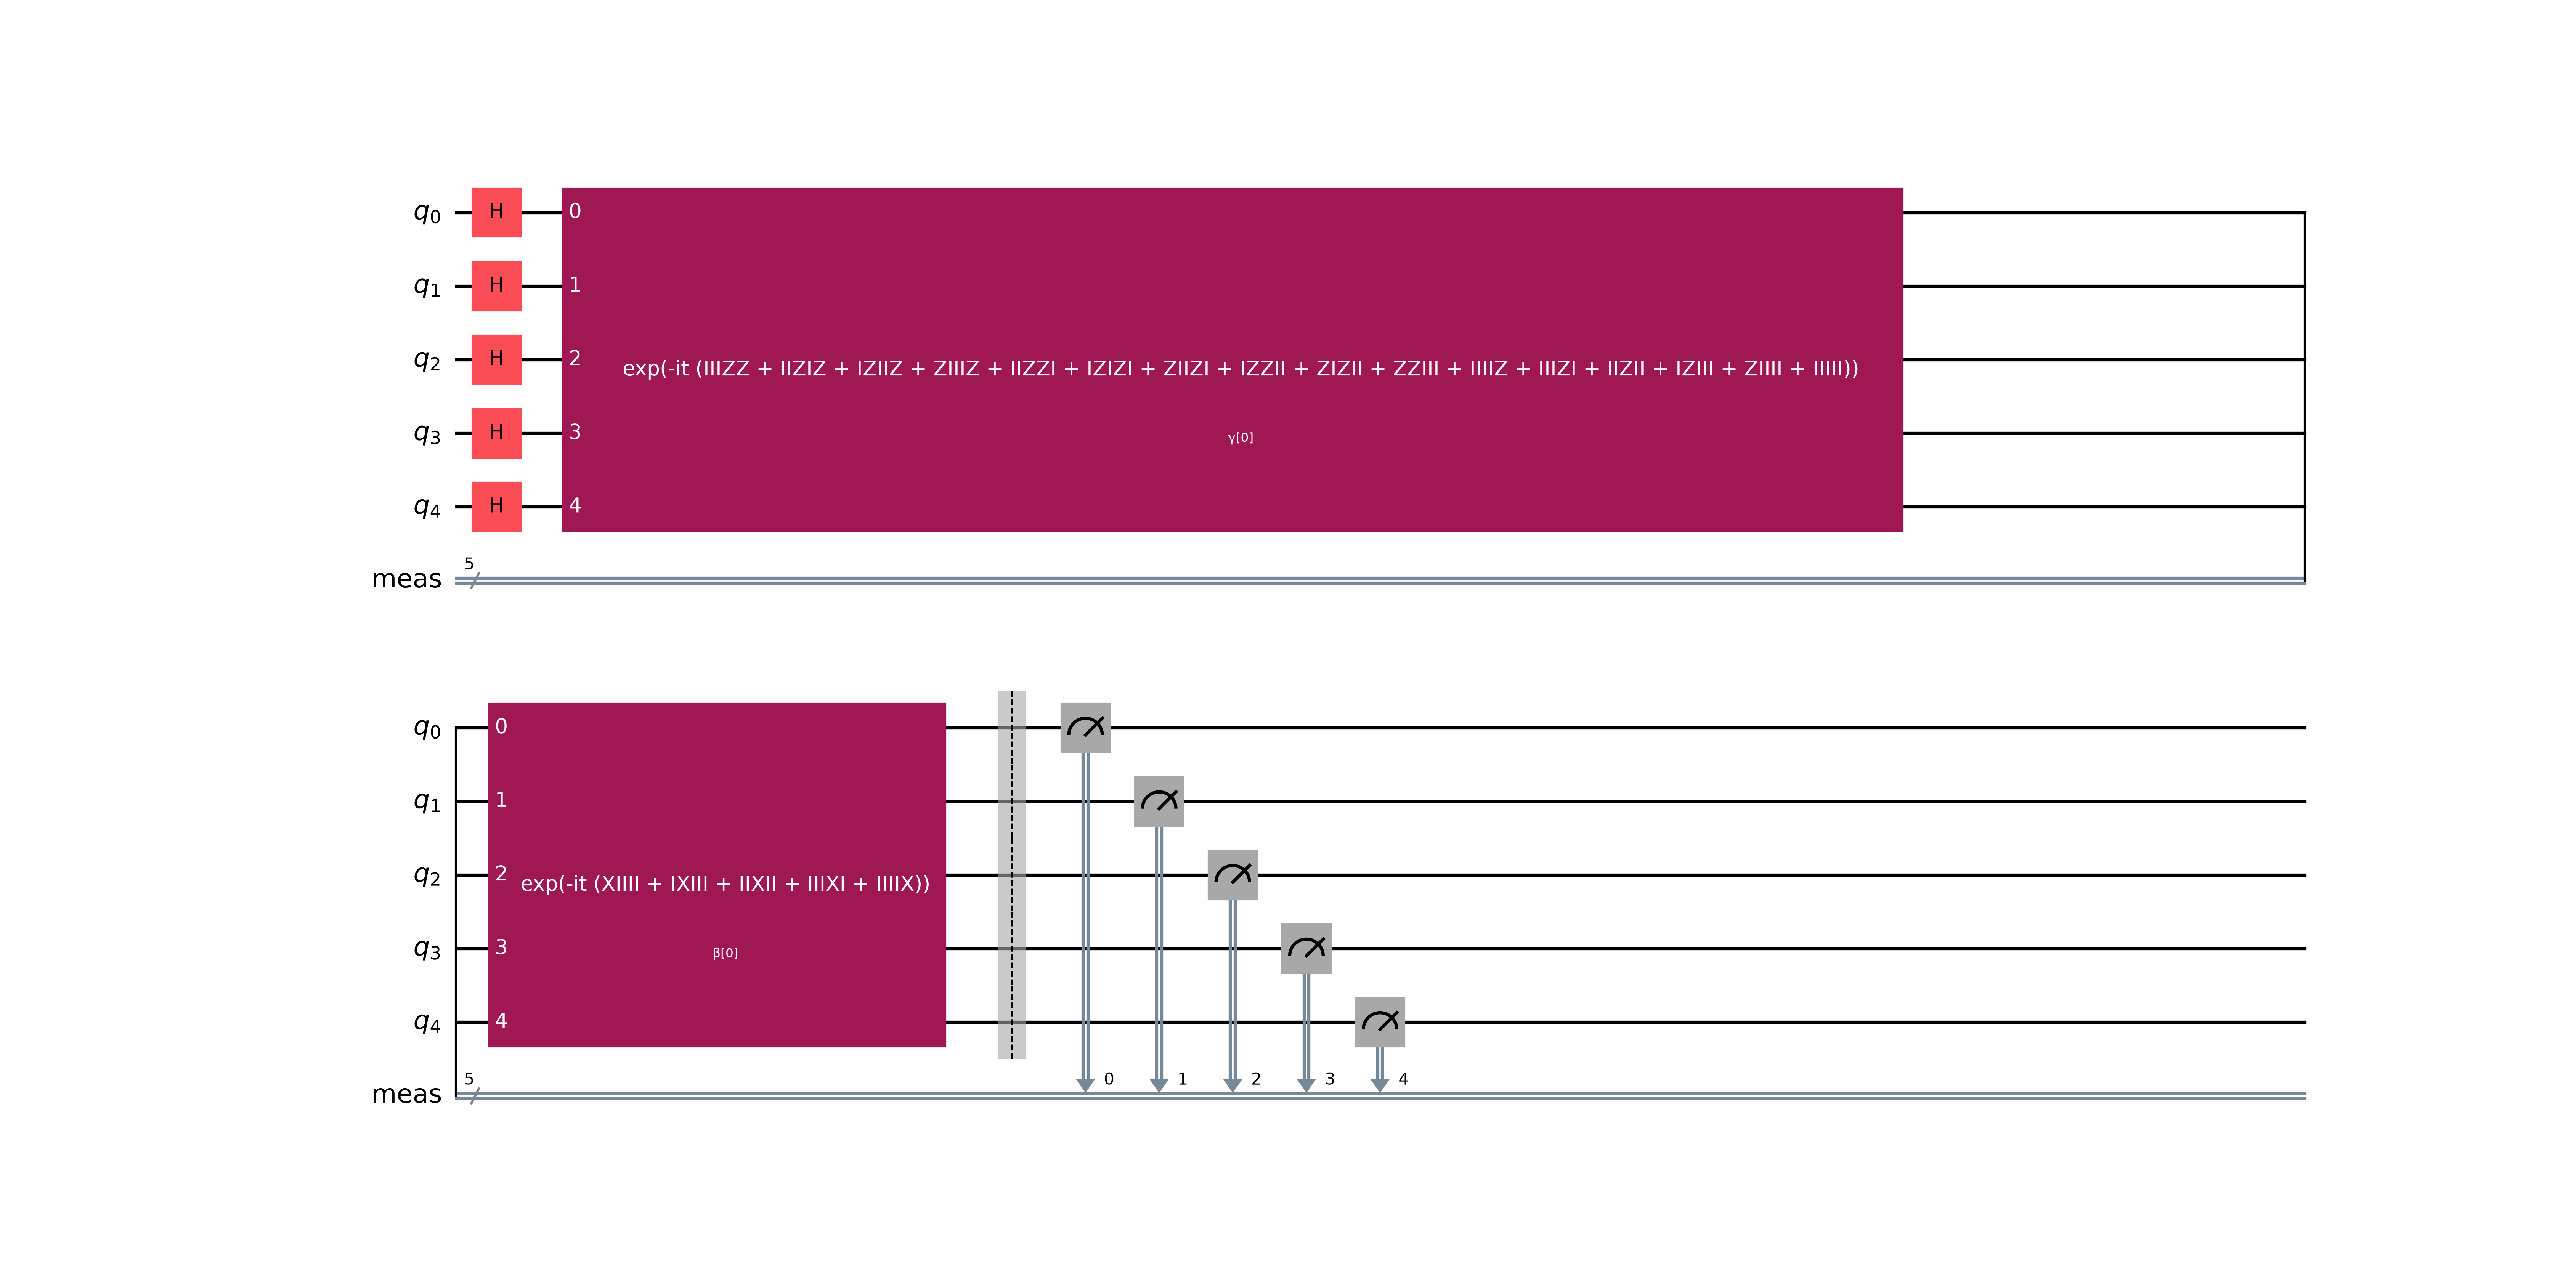
\includegraphics[width=0.85\textwidth]{figures/qaoa_circuit_p1.png}
    \caption{Synthesized QAOA quantum circuit for depth $p=1$ across 5 qubits, depicting initial Hadamard state preparation, entangling two-qubit $ZZ$ phase evolution gates, and single-qubit transverse mixer rotations.}
    \label{fig:qaoa_circuit}
\end{figure}

\section{Ansatz Architecture and Gate Decomposition}
For a chosen depth $p \in \mathbb{N}^+$, the variational ansatz operates on $N$ qubits with $2p$ continuous parameters:
\begin{equation}
\vec{\theta} = (\gamma_1, \dots, \gamma_p, \beta_1, \dots, \beta_p) \in [0, 2\pi]^p \times [0, \pi]^p
\end{equation}

As illustrated in Figure \ref{fig:qaoa_circuit}, each layer $k \in \{1, \dots, p\}$ executes:
\begin{enumerate}
    \item \textbf{Cost Operator Evolution $e^{-i \gamma_k \hat{H}_C}$:}
    Because all terms in $\hat{H}_C$ commute, the operator factorizes without Trotterization error:
    \begin{equation}
    \exp\left(-i \gamma_k \hat{H}_C\right) = \prod_{i < j} \exp\left(-i \gamma_k J_{ij} Z_i Z_j\right) \prod_{i=0}^{N-1} \exp\left(-i \gamma_k h_i Z_i\right)
    \end{equation}
    Each two-qubit interaction term $\exp(-i \gamma_k J_{ij} Z_i Z_j)$ is decomposed into standard native basis gates:
    \begin{equation}
    \text{CNOT}(q_i, q_j) \longrightarrow R_z(2\gamma_k J_{ij}) \text{ on } q_j \longrightarrow \text{CNOT}(q_i, q_j)
    \end{equation}
    requiring $2 \times \binom{N}{2} = N(N-1)$ CNOT gates per layer on an all-to-all connected virtual topology.
    
    \item \textbf{Mixer Evolution $e^{-i \beta_k \hat{H}_B}$:}
    Single-qubit Pauli-$X$ rotations on every qubit:
    \begin{equation}
    \prod_{i=0}^{N-1} R_x(2\beta_k) \text{ on qubit } i
    \end{equation}
\end{enumerate}

\section{Qiskit Primitive Architecture: Estimator vs. Sampler}
Modern Qiskit (version 1.0 through 2.5) decouples quantum execution into two execution primitives:
\begin{enumerate}
    \item \textbf{StatevectorEstimator (Continuous Expectation Value):}
    During the classical optimization loop, evaluating noisy finite-shot estimates of the energy introduces stochastic gradients that degrade deterministic convergence. We employ Qiskit's reference \texttt{StatevectorEstimator}, which computes the exact analytical statevector expectation value:
    \begin{equation}
    \langle \hat{H}_C \rangle = \langle \psi(\vec{\theta}) | \hat{H}_C | \psi(\vec{\theta}) \rangle = \text{Tr}\left( \hat{H}_C |\psi(\vec{\theta})\rangle \langle \psi(\vec{\theta})| \right)
    \end{equation}
    This enables gradient-free and simplex-based classical optimizers to traverse a smooth, deterministic energy surface.
    
    \item \textbf{StatevectorSampler (Multinomial Basis Sampling):}
    Once the optimal variational parameters $\vec{\theta}^* = (\vec{\gamma}^*, \vec{\beta}^*)$ are determined, the quantum state is frozen. To model realistic quantum projective measurement, we attach measurement barriers across all $N$ qubits and invoke \texttt{StatevectorSampler}. Given the final state $|\psi(\vec{\theta}^*)\rangle = \sum_{x} c_x |x\rangle$, the sampler draws $S = 4096$ independent measurement shots from the categorical distribution $P(x) = |c_x|^2$.
\end{enumerate}

\section{Classical Optimization: Powell's COBYLA}
We employ Powell's COBYLA (Constrained Optimization BY Linear Approximation) algorithm \cite{powell1994cobyla}. COBYLA is a derivative-free trust-region simplex method that constructs linear approximations to the objective function at each iteration. It is particularly well suited for low-depth variational landscapes ($2p \le 6$ parameters) where computing numerical finite-difference gradients would require $2 \times 2p$ quantum evaluations per step.

\section{Endianness Decoding and Assignment Mapping}
A critical software pitfall in quantum simulation arises from qubit ordering conventions. Qiskit represents computational basis bitstrings in \textit{little-endian} format: the rightmost character represents qubit 0 (the least significant bit), whereas standard array indexing orders assets left-to-right:
\begin{equation}
\text{Qiskit bitstring: } b_{N-1} b_{N-2} \dots b_1 b_0 \iff x = (b_0, b_1, \dots, b_{N-1})^\top
\end{equation}
Failing to reverse the measurement bitstring inverts asset assignments, leading to erroneous feasibility evaluations and distorted approximation ratios. In our implementation, every measurement key is explicitly decoded and reversed via \texttt{key\_to\_assignment}:
\begin{equation}
x_i = \text{int}(b_{\text{reversed}}[i])
\end{equation}

\section{Formal Evaluation Metrics}
To assess solution quality across classical and quantum solvers, we define three empirical metrics:

\begin{enumerate}
    \item \textbf{Approximation Ratio ($\alpha$):}
    Measures the quality of the best feasible assignment $x_{\text{best}}$ identified by the solver relative to the provable global optimum $x^*$ determined by exhaustive brute-force search:
    \begin{equation}
    \label{eq:approx_ratio}
    \alpha = \frac{\mathcal{U}(x_{\text{best}})}{\mathcal{U}(x^*)}
    \end{equation}
    where $\alpha = 1.0000$ indicates recovery of the global optimum.
    
    \item \textbf{Feasibility Yield ($Y_{\text{feas}}$):}
    Quantifies the percentage of sampled shots that satisfy the strict budget constraint $\sum_{i} x_i = B$:
    \begin{equation}
    \label{eq:feasibility_yield}
    Y_{\text{feas}} = \frac{N_{\text{feasible shots}}}{N_{\text{total shots}}} \times 100\% = \frac{\sum_{x \in \Omega_{\text{feasible}}} \text{Counts}(x)}{S} \times 100\%
    \end{equation}
    In the unoptimized uniform superposition $|+\rangle^{\otimes N}$, the theoretical baseline feasibility yield is purely combinatorial:
    \begin{equation}
    Y_{\text{baseline}} = \frac{\binom{N}{B}}{2^N} \times 100\%
    \end{equation}
    For $N=5$ and $B=2$, $Y_{\text{baseline}} = \frac{10}{32} \times 100\% = 31.25\%$. Any yield $Y_{\text{feas}} > 31.25\%$ proves that constructive quantum interference has shifted probability amplitude into the valid budget subspace.
    
    \item \textbf{Runtime ($t$):}
    Wall-clock execution time measured in seconds using high-resolution monotonic timers (\texttt{time.perf\_counter()}).
\end{enumerate}
